% main.tex — Graduation Thesis
% Zdravoletie / Fontys University of Applied Sciences, 2026
% Author: Alexander Tanev
% Compiler: pdflatex (run twice for references and cross-references)

\documentclass[11pt,a4paper]{report}

% ── Encoding and fonts ─────────────────────────────────────────────────────────
\usepackage[utf8]{inputenc}
\usepackage[T1]{fontenc}
\usepackage{microtype}

% ── Page geometry ──────────────────────────────────────────────────────────────
\usepackage[a4paper, top=2.5cm, bottom=2.5cm, left=2.5cm, right=2.5cm]{geometry}

% ── Headers and footers ────────────────────────────────────────────────────────
\usepackage{fancyhdr}
\pagestyle{fancy}
\fancyhf{}
\fancyhead[L]{\nouppercase{\leftmark}}
\fancyhead[R]{\thepage}
\renewcommand{\headrulewidth}{0.4pt}
\fancypagestyle{plain}{%
  \fancyhf{}
  \fancyhead[R]{\thepage}
  \renewcommand{\headrulewidth}{0.4pt}
}

% ── Tables ─────────────────────────────────────────────────────────────────────
\usepackage{booktabs}
\usepackage{longtable}
\usepackage{array}
\usepackage{graphicx}           % also used for \resizebox on wide tables

% ── Figures ────────────────────────────────────────────────────────────────────
% (graphicx already loaded above)

% ── Mathematics ────────────────────────────────────────────────────────────────
\usepackage{amsmath}

% ── Bibliography ───────────────────────────────────────────────────────────────
\usepackage{natbib}
\bibliographystyle{apalike}

% ── Hyperlinks and PDF metadata ───────────────────────────────────────────────
\usepackage[hidelinks]{hyperref}
\hypersetup{
  pdftitle  = {Reverse-Engineering and Analysis of a Proprietary Health Score},
  pdfauthor = {Alexander Tanev},
}

% ── Spacing ────────────────────────────────────────────────────────────────────
\usepackage{setspace}
\onehalfspacing

% ── Appendix support ──────────────────────────────────────────────────────────
\usepackage[toc,page]{appendix}

% ── Utility ────────────────────────────────────────────────────────────────────
\usepackage{parskip}            % paragraph spacing instead of indent

% ─────────────────────────────────────────────────────────────────────────────
\begin{document}

% ── Title page ────────────────────────────────────────────────────────────────
\begin{titlepage}
  \centering
  \vspace*{2cm}
  {\LARGE\bfseries Reverse-Engineering and Analysis of a Proprietary Health Score\\
  from Raw Biometric Inputs\par}
  \vspace{1.5cm}
  {\large Comparative Evaluation of Modelling Approaches and\\
  Synthetic Data Augmentation\par}
  \vspace{2cm}
  {\large Alexander Tanev\par}
  \vspace{0.5cm}
  {\normalsize BSc Applied Mathematics, Data Science\par}
  {\normalsize Fontys University of Applied Sciences\par}
  \vspace{1cm}
  {\normalsize Internship at Zdravoletie Health and Rehabilitation Centre,\\
  Varna, Bulgaria\par}
  \vspace{1cm}
  {\normalsize Company supervisor: Kostadin Galchin\par}
  {\normalsize Educational supervisor: Peter Alem\par}
  \vspace{2cm}
  {\normalsize June 2026\par}
  \vfill
\end{titlepage}

% ── Abstract ──────────────────────────────────────────────────────────────────
\newpage
\thispagestyle{plain}
\chapter*{Abstract}
\addcontentsline{toc}{chapter}{Abstract}

Commercial body scanning platforms such as Anovator produce proprietary composite health scores
whose computational basis is undisclosed. This study treats the Anovator bodyAge score as a
reverse-engineering target rather than a validated clinical measure, asking whether machine
learning regression models can learn to reproduce it from the raw biometric inputs the platform
records. The target variable is the age gap, defined as bodyAge minus chronological age. Data
comprise 158 scan records from 53 unique clients collected at Zdravoletie, a health and
rehabilitation centre in Bulgaria.

Three experiments were conducted using 30 repeated GroupShuffleSplit cross-validation iterations
grouped by client identity. Experiment~1 compared five regressors --- RandomForest, Ridge, SVR,
GradientBoosting, and HistGradientBoosting --- on the full 88-feature set. HistGradientBoosting
achieved the lowest mean MAE of 2.43 years (95\% CI [2.09, 2.76]), but none of the ten pairwise
Wilcoxon signed-rank tests reached the Bonferroni-corrected significance threshold of 0.005; all
model comparisons are inconclusive at this sample size. Experiment~2 tested three training
regimes --- real data only, real plus 1000 GMM-generated synthetic records, and synthetic only ---
finding that synthetic augmentation significantly reduced MAE for four of five models (adjusted
$p < 0.003$) but degraded Ridge under the synthetic-only condition from 2.48 to 3.23 years, a
consequence of pseudo-label variance compression that does not affect tree-based methods.
Experiment~3 evaluated four cumulative feature groups using HistGradientBoosting, finding that
the 63-feature anthropometric and metabolic base group alone achieved the lowest mean MAE of 2.39
years, with no statistically significant improvement from adding bioimpedance, postural risk, or
joint angle features --- suggesting these modalities carry negligible independent weight in the
Anovator formula at this data scale.

The primary limitation is dataset size: 53 individuals is insufficient for high-power pairwise
significance testing after Bonferroni correction, and most comparisons must be characterised as
inconclusive rather than resolved.

\newpage

% ── Table of contents ─────────────────────────────────────────────────────────
\tableofcontents
\newpage

% ── List of figures ───────────────────────────────────────────────────────────
\listoffigures
\newpage

% ── List of tables ────────────────────────────────────────────────────────────
\listoftables
\newpage

% =============================================================================
\chapter{Introduction}
% =============================================================================

\section{Research Context}

The past decade has seen a proliferation of commercial health assessment platforms that transform
raw biometric measurements into composite health scores intended for use in wellness,
rehabilitation, and preventive health contexts. These platforms --- combining bioelectrical
impedance analysis, postural imaging, anthropometric measurement, and proprietary scoring
algorithms --- are deployed in gyms, clinics, and corporate health programmes, where their outputs
are presented to clients and practitioners as meaningful summaries of physiological condition. The
Anovator body scanning system, used in this study, is representative of this category: it produces
a score called bodyAge, expressed as an estimated biological age in years, derived from a
combination of body composition, postural, impedance, and biometric inputs through an undisclosed
computational formula.

The interpretability gap created by this architecture is practically significant. A client whose
Anovator scan returns a bodyAge five years above their chronological age has been told something
consequential about their health, but neither the client nor the attending practitioner can inspect
the mechanism that produced this number. Which measurements contributed most to the result? Is the
score driven primarily by body fat distribution, postural risk, or impedance characteristics? How
would a change in a specific biometric --- achieved through a targeted intervention --- translate
into a change in the score? Without access to the proprietary formula, none of these questions can
be answered by examining the score alone. This is not unique to Anovator: the same interpretability
gap exists across the broader class of commercial health scoring devices, and it limits the
evidential value of their outputs for clinical reasoning.

\section{Research Question}

This project addresses that gap through a reverse-engineering approach. Rather than predicting
biological age in the clinical sense --- where ground truth is established against mortality or
morbidity endpoints, as in the biological age literature reviewed in Chapter~\ref{chap:related} ---
the study treats the Anovator bodyAge score itself as the target variable and asks whether machine
learning regression models can learn to reproduce it from the raw biometric inputs that the Anovator
system records. The age gap, defined as bodyAge minus chronological age, is used as the prediction
target throughout in order to remove the trivial component of chronological age from the target
distribution and focus modelling effort on the physiological deviation component that the Anovator
formula computes.

Three research sub-questions guide the empirical work. First: among five regression algorithms
spanning linear, kernel, and ensemble methods, which best approximates the Anovator age gap from
the full feature set, and can any observed differences between models be established as statistically
significant given the available data? Second: does augmenting the training set with synthetic records
generated by a Gaussian Mixture Model and pseudo-labelled by the production model improve
approximation quality on real held-out data, and if so, for which model classes? Third: across four
cumulative groups of biometric features --- anthropometric and metabolic measurements, bioimpedance,
postural risk scores, and joint angles --- which groups carry independent predictive information
relative to the Anovator score, and which are redundant with what the base group already provides?

\section{Study Design and Scope}

The empirical programme comprises three experiments conducted on a dataset of 158 Anovator scan
records drawn from 53 unique clients at Zdravoletie, a health and rehabilitation centre in Varna,
Bulgaria. Data were collected between 2022 and 2024. All experiments use 30 repeated
GroupShuffleSplit cross-validation iterations grouped by client identity to prevent person-level data
leakage, and report performance as mean error with 95\% confidence intervals. Statistical
significance between conditions is assessed using the Wilcoxon signed-rank test with Bonferroni
correction for multiple comparisons.

The scope of the project is deliberately constrained. It covers exactly the three experiments
described above. What lies outside the scope is equally important to state clearly. This project
does not attempt to validate the Anovator bodyAge score as a clinical measure of biological ageing;
the absence of an independently validated ground truth makes such validation impossible within this
dataset, and the research question does not require it. The study does not investigate alternative
synthetic data generation methods beyond the Gaussian Mixture Model --- CTGAN, vine copula, and
variational autoencoder approaches are noted in the related work but excluded from empirical
comparison on the grounds that the 158-record training corpus falls below the regime in which these
methods train reliably without extensive hyperparameter search. The study does not explore
time-based train-test splits, as the dataset contains insufficient longitudinal density per
individual to make temporal generalisation the primary evaluation criterion. These exclusions are
not omissions; they are boundaries that keep the empirical claims within what the data can support.

\section{Practical Significance}

Understanding the informational structure of a proprietary health score has concrete value even in
the absence of access to the formula itself. If reverse-engineering experiments reveal that the
anthropometric and metabolic feature group alone accounts for essentially all predictable variation
in the Anovator bodyAge score --- as Experiment~3 suggests --- then practitioners can infer that the
specialised measurement modalities contribute negligible marginal information to the score and focus
their interpretive attention accordingly. More broadly, the methodology developed here --- reverse-engineering
a proprietary score through grouped cross-validation, statistical significance testing under multiple
comparisons, and feature group ablation --- is transferable to any context in which a commercial health
device produces a black-box output that practitioners wish to understand without access to the
underlying formula.


% =============================================================================
\chapter{Related Work}
\label{chap:related}
% =============================================================================

\section{Biological Age Prediction}

The quantification of biological age --- an individual's physiological age as distinct from their
chronological age --- has been an active area of research in gerontology and clinical epidemiology
for several decades. Early attempts used simple composite indices of physical performance or blood
chemistry, but the foundational theoretical treatment of the problem was provided by
\citet{Klemera2006}, who formalised biological age estimation as a regression problem in which the
true biological age is treated as a latent variable estimated from a set of biomarkers. Their method
fits a collection of simple linear regressions, one per biomarker, modelling each biomarker as a
function of chronological age, and then combines these fits into a composite biological age estimate
that is optimal in the sense of minimising the mean squared distance between the estimated biological
age and the biomarker values. \citet{Klemera2006} demonstrated that their method produces lower
estimation error than earlier composite approaches and explicitly accounts for the fact that
biomarkers have different slopes and residual variances with respect to chronological age.

The field advanced substantially with the development of epigenetic clocks, which exploit the
observation that DNA methylation at specific CpG sites in the genome changes in a highly
age-predictable manner across tissue types. \citet{Horvath2013} demonstrated that a penalised
regression model trained on methylation data from 51 tissue types could predict chronological age
with a median absolute error of approximately 3.6 years and that systematic deviations from the
predicted age --- termed age acceleration --- were associated with disease status and mortality risk.
Building on this foundation, \citet{Levine2018} introduced PhenoAge, a composite biological age
measure derived from nine clinical blood biomarkers combined with chronological age through a
Gompertz proportional hazards model trained on mortality data from the National Health and Nutrition
Examination Survey. The defining feature of PhenoAge is that it is calibrated against a mortality
endpoint: a PhenoAge that exceeds chronological age carries a validated association with elevated
all-cause mortality risk. \citet{Lu2019} extended this line of work with GrimAge, an epigenetic
clock trained on plasma protein levels and smoking pack-years via DNA methylation proxies, optimised
to predict time-to-death. GrimAge demonstrated substantially stronger associations with lifespan and
health outcomes than earlier methylation clocks.

The present project differs from this literature in both the ground truth available and the
measurement modalities used. The ground truth is not a clinical endpoint but the proprietary bodyAge
score computed by the Anovator scanning platform. The research question is accordingly not whether
a model can predict how quickly an individual will age in a clinical sense, but whether a model can
learn to reproduce the Anovator formula's output from its inputs --- a reverse-engineering problem.

\section{Synthetic Data Generation in Small Medical Datasets}

The scarcity of labelled data is a recurring constraint in medical machine learning, where data
collection is costly, privacy regulations limit sharing, and cohort sizes at individual institutions
are often in the hundreds rather than the thousands.

The earliest and most widely used approach in the context of class imbalance is SMOTE, introduced
by \citet{Chawla2002}, which generates new minority-class instances by interpolating between
existing instances in feature space. SMOTE operates in a purely local neighbourhood context and
does not model the global joint distribution of features.

Gaussian Mixture Models fit a weighted sum of multivariate Gaussian distributions to the observed
data and generate synthetic samples by drawing from the fitted mixture. GMMs are computationally
efficient, produce closed-form likelihood estimates, and require relatively few observations to fit
stably --- properties that make them well suited to small tabular datasets in the low-hundreds-of-records
regime.

\citet{Xu2019} introduced CTGAN, a Conditional Generative Adversarial Network specifically designed
for tabular data, addressing multi-modal non-Gaussian distributions and class imbalance through
mode-specific normalisation and conditional generation. However, GAN training is sensitive to the
ratio of training samples to model parameters, and mode collapse becomes substantially more likely
when training sample sizes fall below approximately one thousand records per class.

Copula-based approaches, as systematised in the Synthetic Data Vault framework by \citet{Patki2016},
model the joint distribution by separately estimating each variable's marginal distribution and using
a copula to capture the dependence structure. For this project, a five-component Gaussian Mixture
Model with full covariance matrices was selected as the synthesis method on the grounds of suitability
to the dataset scale of 158 records.

\section{Feature Importance and Interpretability in Health Machine Learning}

The deployment of machine learning models in health-related contexts introduces an obligation of
interpretability that is distinct from the pure predictive performance requirements of general
machine learning applications.

The SHapley Additive exPlanations framework, introduced by \citet{Lundberg2017}, provides a
theoretically grounded approach to feature attribution. SHAP values are derived from cooperative
game theory: the contribution of each feature to a particular prediction is computed as the average
marginal contribution of that feature across all possible orderings in which features are added to
the model. This foundation gives SHAP values three properties that competing attribution methods do
not simultaneously satisfy: local accuracy, consistency, and missingness.

\citet{Lundberg2020} developed TreeSHAP, an algorithm that exploits the structure of tree-based
ensemble models to compute exact SHAP values in polynomial time, making SHAP analysis
computationally feasible for random forests and gradient boosting models. In a landmark clinical
application, \citet{Lundberg2018} used SHAP explanations to identify the features driving a gradient
boosting model's predictions of sepsis onset in intensive care patients, demonstrating that SHAP
could surface clinically meaningful feature importance patterns that were subsequently validated by
domain experts.

In the present project, SHAP analysis serves two purposes. Globally, summary plots of mean absolute
SHAP values provide an empirical ranking of feature importance that complements Experiment~3. Locally,
force plots decompose individual predictions into feature contributions, providing the interpretable
patient-level output displayed in the Zdravoletie Streamlit dashboard. It should be noted that SHAP
values explain the model's behaviour, not the underlying physiological process: they characterise
the information structure of the Anovator score as recovered by the model, subject to the
approximation error and feature encoding limitations described in Chapter~\ref{chap:method}.


% =============================================================================
\chapter{Methodology}
\label{chap:method}
% =============================================================================

\section{Thesis Framing and Research Objective}

This project does not aim to predict biological age in the general sense. Its specific objective is
to reverse-engineer and analyse Anovator's proprietary bodyAge score from raw biometric inputs, and
to evaluate three dimensions of that modelling problem: which regression algorithm best approximates
the score, whether Gaussian Mixture Model synthetic data augmentation improves approximation quality,
and which biometric feature groups carry the most predictive information relative to the score.

\section{Dataset}

\subsection{Source and Collection}

All data originate from Anovator body scan sessions conducted at Zdravoletie, a health and
rehabilitation centre in Bulgaria. Records were collected between 2022 and 2024 using the Anovator
scanning platform, which combines impedance bioelectrical analysis, postural camera imaging, and
manual biometric measurements. The dataset comprises 158 individual scan records drawn from 53
unique clients, with each client potentially appearing in multiple records across different sessions.
The dataset was assembled manually from the Anovator web interface; no public data sources were
combined with it.

\subsection{Target Variable}

Anovator computes a proprietary score called bodyAge for each scan. The target variable throughout
all experiments is the age gap, defined as the signed difference between bodyAge and the client's
chronological age at the time of the scan:

\begin{equation}
  \text{age\_gap} = \text{bodyAge} - \text{age}
\end{equation}

A positive age\_gap indicates that the Anovator system judged the client's biological condition to
be older than their chronological age; a negative value indicates the reverse. Across the 158
records, age\_gap has a mean of 0.45 years and a standard deviation of 3.30 years.

\subsection{Feature Set}

The final model feature set comprises 88 variables derived from the raw Anovator outputs, decomposed
into four groups used in Experiment~3.

\textbf{Group 1 --- Anthropometric and metabolic (63 features):} Body composition measurements
(weight, height, BMI, body fat percentage, muscle mass, bone mass, protein content, water content,
subcutaneous fat, intra-abdominal fat, and segmental decompositions), Anovator-computed health goal
recommendations, balance and agility scores, vital signs where available, and demographic features.

\textbf{Group 2 --- Bioimpedance (10 features):} Raw impedance measurements at 20\,kHz and 100\,kHz
for each of the four limbs and the trunk
(\texttt{r20LeftArm}, \texttt{r20RightArm}, \texttt{r20LeftLeg}, \texttt{r20RightLeg},
\texttt{r20Trunk}, \texttt{r100LeftArm}, \texttt{r100RightArm}, \texttt{r100LeftLeg},
\texttt{r100RightLeg}, \texttt{r100Trunk}).

\textbf{Group 3 --- Postural risk (10 features):} Camera-based postural risk scores
(\texttt{frontHeadRisk}, \texttt{headRisk}, \texttt{humpbackRisk}, \texttt{kneeRisk},
\texttt{pelvisRisk}, \texttt{postureRisk}, \texttt{shoulderRisk}, \texttt{spineRisk},
\texttt{side\_hunchback\_risk}) and a derived aggregate (\texttt{aggregated\_postural\_index}).

\textbf{Group 4 --- Joint angles (5 features):} \texttt{front\_shoulder\_angle},
\texttt{front\_left\_leg\_angle}, \texttt{front\_right\_leg\_angle},
\texttt{side\_left\_leg\_angle}, \texttt{side\_right\_leg\_angle}.

\section{Feature Engineering}

Five derived features are computed from raw columns. Sex is encoded as a binary integer (0 for
female, 1 for male). Three body composition ratios are computed: muscle-to-fat ratio (muscle divided
by fat plus 0.1), upper-to-lower body muscle ratio (upperBody divided by lowerBody plus 0.1), and
trunk-to-limb fat ratio (fatTrunk divided by the sum of the four limb fat measurements plus 0.1).
The additive constant of 0.1 in each denominator prevents division by zero and is applied
consistently across all contexts. The \texttt{aggregated\_postural\_index} is the mean of
\texttt{humpbackRisk}, \texttt{spineRisk}, \texttt{pelvisRisk}, \texttt{postureRisk},
\texttt{kneeRisk}, and \texttt{frontHeadRisk}.

\section{Cross-Validation Protocol}

\subsection{Group-Based Splitting}

All three experiments use \texttt{GroupShuffleSplit} from scikit-learn with the grouping variable
set to the client name field. This prevents data leakage at the person level: all of a given
client's records are assigned together to either the training fold or the test fold. Without this
constraint, a model could exploit within-person consistency --- learning the stable biometric profile
of an individual --- rather than generalising across individuals, which would inflate performance
estimates.

Each split assigns 80\% of the 53 unique individuals to training and 20\% to test, yielding
approximately 11 to 13 test records per split. The split is non-exhaustive and repeated 30 times.
All splits use a fixed random seed of 42.

\subsection{Imputation and Scaling}

Missing values are imputed using the median of the training fold in each split, computed fresh from
the training fold after the split is drawn. A secondary \texttt{fillna(0)} handles the rare case
where a feature is entirely missing from the training fold. The test fold is imputed using the same
training-fold medians --- ensuring that no information from the test set informs the imputation.
\texttt{StandardScaler} is fit on the training fold after imputation and applied to both folds.

\section{Experiment 1: Model Comparison}

Experiment~1 evaluates five regression algorithms: \texttt{RandomForestRegressor}, \texttt{Ridge},
\texttt{SVR} (radial basis function kernel), \texttt{GradientBoostingRegressor}, and
\texttt{HistGradientBoostingRegressor}. All models use scikit-learn implementations with fixed
hyperparameters specified in a central configuration module. RandomForest uses 100 estimators with
maximum depth 7. Ridge uses a regularisation coefficient of 1.0. SVR uses a radial basis function
kernel with $C=1.0$ and $\varepsilon=0.1$. GradientBoosting uses 100 estimators with learning rate
0.1 and maximum depth 3. HistGradientBoosting uses 100 maximum iterations.

For each of the 30 splits, fresh model instances are trained on the scaled training fold and
evaluated on the scaled test fold. MAE, RMSE, and $R^2$ are recorded for each model in each split,
yielding 30 paired observations per model. Summary statistics (mean, standard deviation, and 95\%
confidence interval) are computed using the $t$-distribution with 29 degrees of freedom.

\section{Experiment 2: Synthetic Data Ablation}

Experiment~2 investigates whether augmenting the training set with GMM synthetic data improves
prediction of age\_gap on real held-out data. Three training regimes are evaluated for each of the
five models:

\begin{itemize}
  \item \textbf{RealOnly}: trains exclusively on the real records in the training fold.
  \item \textbf{RealPlusSynth}: augments the real training fold with all 1000 synthetic records
    before training.
  \item \textbf{SynthOnly}: trains exclusively on the 1000 synthetic records and evaluates on the
    real test fold.
\end{itemize}

The 1000-record synthetic dataset was generated by fitting a Gaussian Mixture Model with five
components and full covariance matrices to the 158 real records. Pseudo-labels were generated by
applying the production model (trained on all 158 real records) to the synthetic feature vectors,
constituting a teacher-student knowledge distillation setup. The pseudo-labels have a mean of
0.75 years and a standard deviation of 1.91 years, compared to the real label distribution of mean
0.45 years and standard deviation 3.30 years.

\section{Experiment 3: Feature Group Ablation}

Experiment~3 evaluates the marginal contribution of each biometric feature group using
HistGradientBoosting as the sole model. Feature groups are evaluated cumulatively:

\begin{itemize}
  \item Group 1 (63 features): anthropometric and metabolic features only.
  \item Group 2 (73 features): Group 1 plus ten bioimpedance measurements.
  \item Group 3 (83 features): Group 2 plus ten postural risk scores.
  \item Group 4 (88 features): Group 3 plus five joint angle measurements.
\end{itemize}

The same 30-split protocol, imputation procedure, and scaling procedure apply.

\section{Statistical Testing}

Pairwise statistical significance is assessed using the Wilcoxon signed-rank test, appropriate for
paired, non-normally distributed observations. In Experiment~1, the $C(5,2) = 10$ model pairs yield
a corrected significance threshold of $\alpha = 0.005$ after Bonferroni correction. In
Experiment~2, three regime pairs per model yield a corrected threshold of $\alpha/3 \approx 0.0167$.
In Experiment~3, six group pairs yield a corrected threshold of $\alpha/6 \approx 0.0083$.

A result that does not reach the corrected significance threshold must be characterised as
inconclusive rather than as evidence of equivalence. With 30 paired observations and a corrected
threshold well below the nominal 0.05 level, the tests have limited statistical power to detect
moderate effect sizes.

\section{Known Limitations of the Dataset and Feature Set}
\label{sec:limitations}

\subsection{Sentinel Values Encoded as Numeric Features}

Two features use the integer $-1$ as a machine sentinel meaning that the metric was not computed
for a given scan: \texttt{sportSafeRisk} is $-1$ in 37\% of records and \texttt{sportLevel} is
$-1$ in 70\% of records. Both features are included in the model feature set and are passed to all
models as continuous numeric inputs. Proper encoding --- replacing $-1$ with \texttt{NaN} followed
by indicator-variable encoding and imputation --- is listed in future work.

\subsection{Near-Constant Features After Median Imputation}

Five features have missingness rates exceeding 88\% of records: \texttt{leftVision} (94.3\%),
\texttt{rightVision} (92.4\%), \texttt{bloodMaxPressure} (91.8\%), \texttt{bloodMinPressure}
(91.8\%), and \texttt{restingHeartRate} (88.6\%). After training-set median imputation, these
features take a single constant value for the majority of records in any given training fold,
contributing negligible variance and therefore negligible predictive signal.

\subsection{Redundant Derived Feature Within the Postural Risk Group}

The feature \texttt{aggregated\_postural\_index} is the arithmetic mean of six postural risk scores
that are themselves present as individual variables in the same feature group. The aggregate carries
no independent information relative to its components when all six are simultaneously available.

\subsection{Statistical Power of the Wilcoxon Test Under Bonferroni Correction}
\label{sec:power}

At 30 paired observations and a corrected $\alpha$ of 0.005, the Wilcoxon signed-rank test has
limited power to detect moderate effect sizes in the range of Cohen's $d = 0.3$ to 0.5. The root
cause is the dataset size: 53 unique individuals is insufficient for high-power pairwise testing
after Bonferroni correction.


% =============================================================================
\chapter{Results}
% =============================================================================

\section{Preliminary Note on \texorpdfstring{$R^2$}{R-squared}}

All three experiments report mean $R^2$ alongside MAE and RMSE for completeness. However, $R^2$
must be interpreted with caution: each test fold contains between 11 and 13 records, and with test
sets of this size $R^2$ estimates are extremely noisy. All five models return negative mean $R^2$
values in the RealOnly regime of Experiment~2, a consequence of evaluating on 11--13 rows with high
outcome variance (age\_gap standard deviation = 3.30 years). MAE and RMSE are the primary metrics
throughout; $R^2$ results are reported for completeness and transparency but are not used as the
basis for any comparative claims.

\section{Experiment 1: Model Comparison}

\subsection{Performance Across Metrics}

Table~\ref{tab:exp1_results} presents mean MAE, RMSE, and $R^2$ with 95\% confidence intervals
for all five models, derived from 30 GroupShuffleSplit folds.

\begin{table}[h]
  \centering
  \caption{Experiment 1: Mean performance metrics (95\% CI) across 30 folds. Models ordered by
  ascending mean MAE.}
  \label{tab:exp1_results}
  \small
  \resizebox{\textwidth}{!}{%
  \begin{tabular}{lrrrrrr}
    \toprule
    \textbf{Model} & \textbf{MAE mean} & \textbf{MAE 95\% CI}
                   & \textbf{RMSE mean} & \textbf{RMSE 95\% CI}
                   & \textbf{$R^2$ mean} & \textbf{$R^2$ 95\% CI} \\
    \midrule
    HistGradientBoosting & 2.43 & [2.09,\ 2.76] & 3.05 & [2.66,\ 3.44] & $-0.36$ & [$-0.70$,\ $-0.03$] \\
    Ridge                & 2.48 & [2.09,\ 2.87] & 3.10 & [2.62,\ 3.58] & $-0.49$ & [$-1.06$,\ 0.08] \\
    RandomForest         & 2.51 & [2.18,\ 2.84] & 3.20 & [2.85,\ 3.56] & $-0.47$ & [$-0.77$,\ $-0.17$] \\
    GradientBoosting     & 2.51 & [2.19,\ 2.84] & 3.13 & [2.75,\ 3.51] & $-0.42$ & [$-0.74$,\ $-0.10$] \\
    SVR                  & 2.62 & [2.30,\ 2.94] & 3.42 & [3.11,\ 3.73] & $-0.66$ & [$-0.91$,\ $-0.41$] \\
    \bottomrule
  \end{tabular}}
\end{table}

\begin{figure}[h]
  \centering
  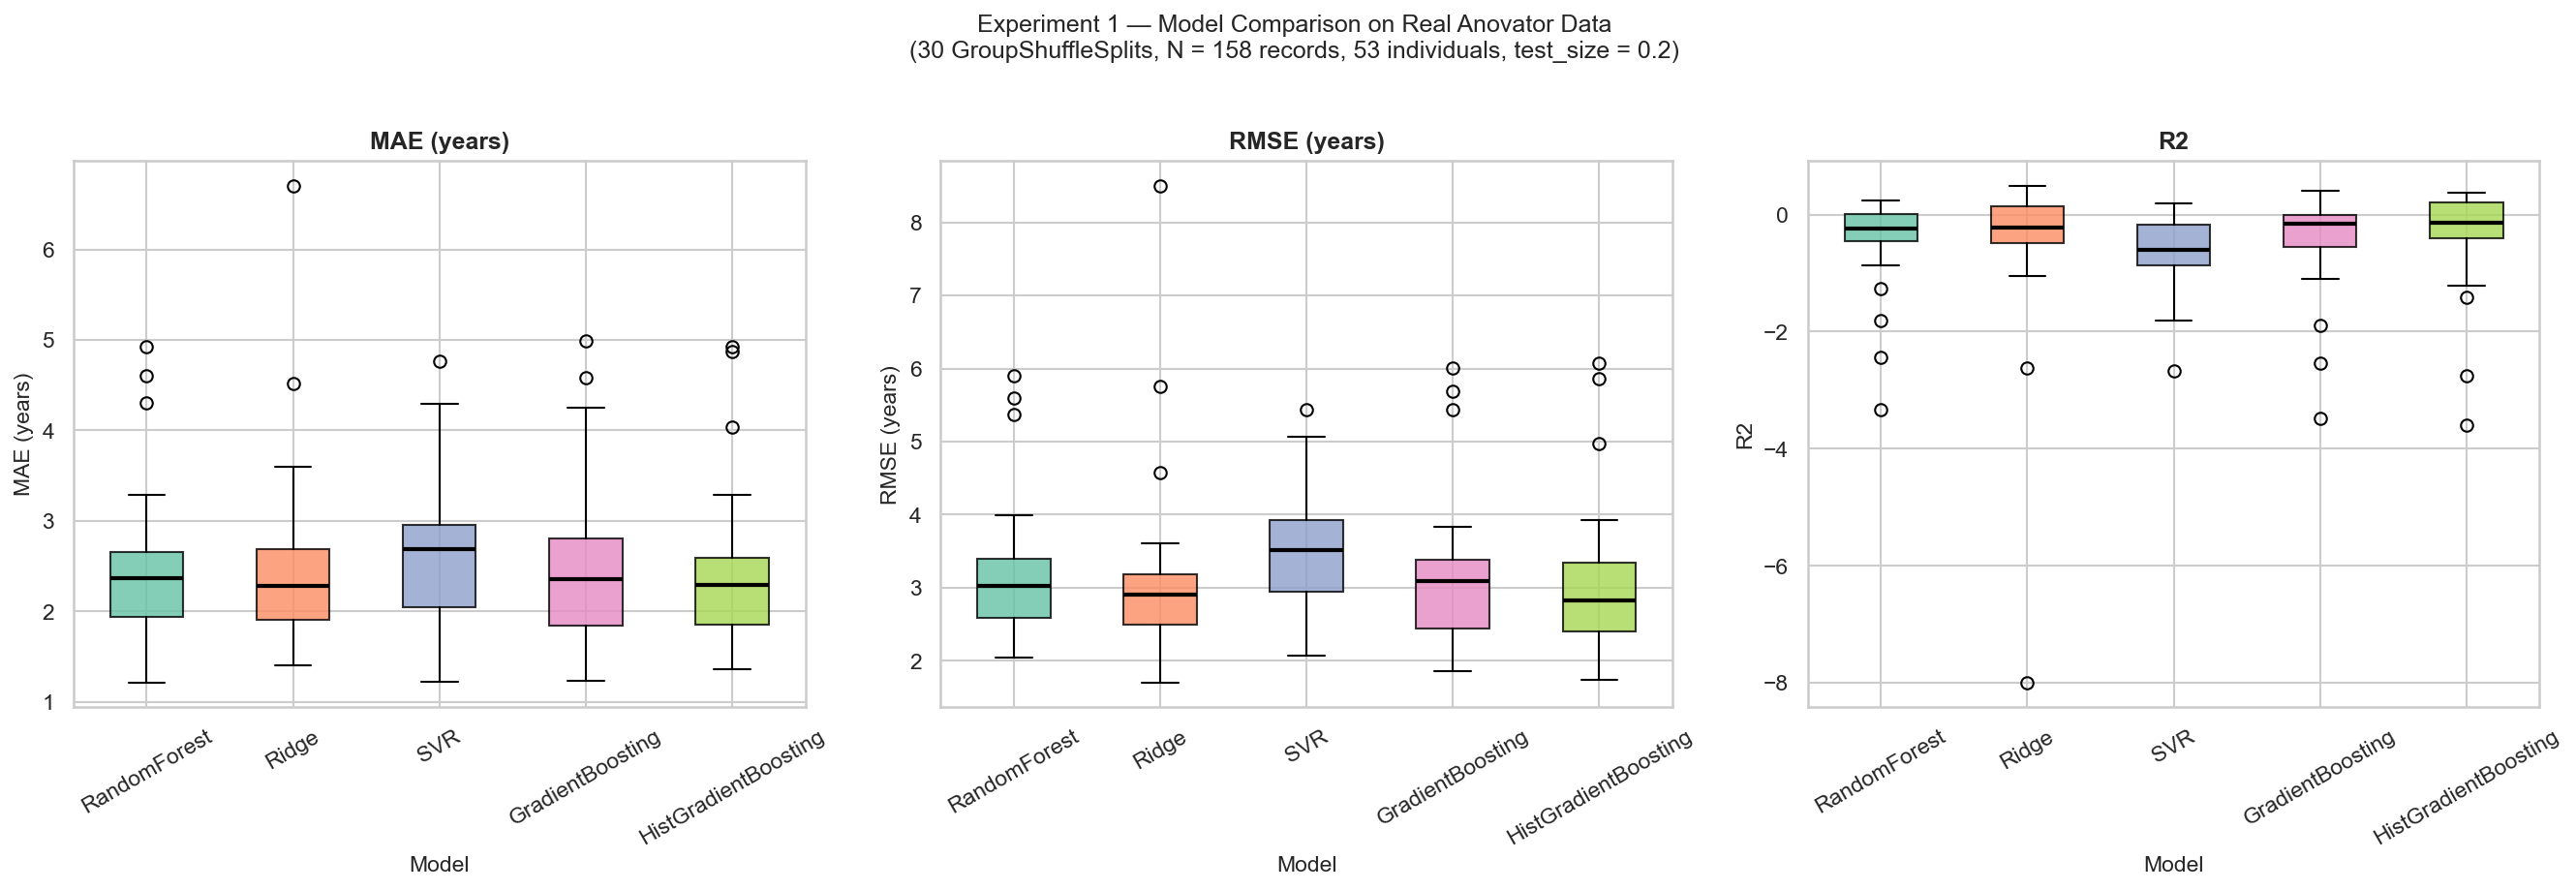
\includegraphics[width=0.85\textwidth]{../results/experiment_1_boxplot.png}
  \caption{Box plot of MAE distributions across 30 cross-validation folds for all five models
  (Experiment~1). Models are ordered by ascending median MAE. The horizontal line within each box
  represents the median; the box spans the interquartile range; whiskers extend to 1.5 times the
  IQR.}
  \label{fig:exp1_boxplot}
\end{figure}

HistGradientBoosting achieves the lowest mean MAE at 2.43 years and the lowest mean RMSE at 3.05
years. SVR has the highest mean MAE at 2.62 years. The 95\% confidence intervals for MAE overlap
extensively across all five models, consistent with the significance test results in
Section~\ref{sec:exp1_sig}.

\subsection{Statistical Significance}
\label{sec:exp1_sig}

Table~\ref{tab:exp1_sig} presents the Wilcoxon signed-rank test results for all ten model pairs on
MAE, with Bonferroni-corrected $p$-values and the corrected significance threshold of 0.005.

\begin{table}[h]
  \centering
  \caption{Experiment 1: Wilcoxon signed-rank test results for MAE (Bonferroni $\alpha = 0.005$).}
  \label{tab:exp1_sig}
  \begin{tabular}{llrrr}
    \toprule
    \textbf{Model A} & \textbf{Model B} & \textbf{$p$ (raw)} & \textbf{$p$ (adjusted)} & \textbf{Significant} \\
    \midrule
    SVR              & HistGradientBoosting & 0.0043 & 0.0434 & No \\
    RandomForest     & HistGradientBoosting & 0.0577 & 0.5769 & No \\
    RandomForest     & SVR                  & 0.0636 & 0.6356 & No \\
    Ridge            & SVR                  & 0.0767 & 0.7672 & No \\
    GradientBoosting & HistGradientBoosting & 0.1294 & 1.0000 & No \\
    RandomForest     & Ridge                & 0.2710 & 1.0000 & No \\
    Ridge            & GradientBoosting     & 0.2710 & 1.0000 & No \\
    SVR              & GradientBoosting     & 0.3599 & 1.0000 & No \\
    RandomForest     & GradientBoosting     & 0.8236 & 1.0000 & No \\
    Ridge            & HistGradientBoosting & 0.9515 & 1.0000 & No \\
    \bottomrule
  \end{tabular}
\end{table}

\begin{figure}[h]
  \centering
  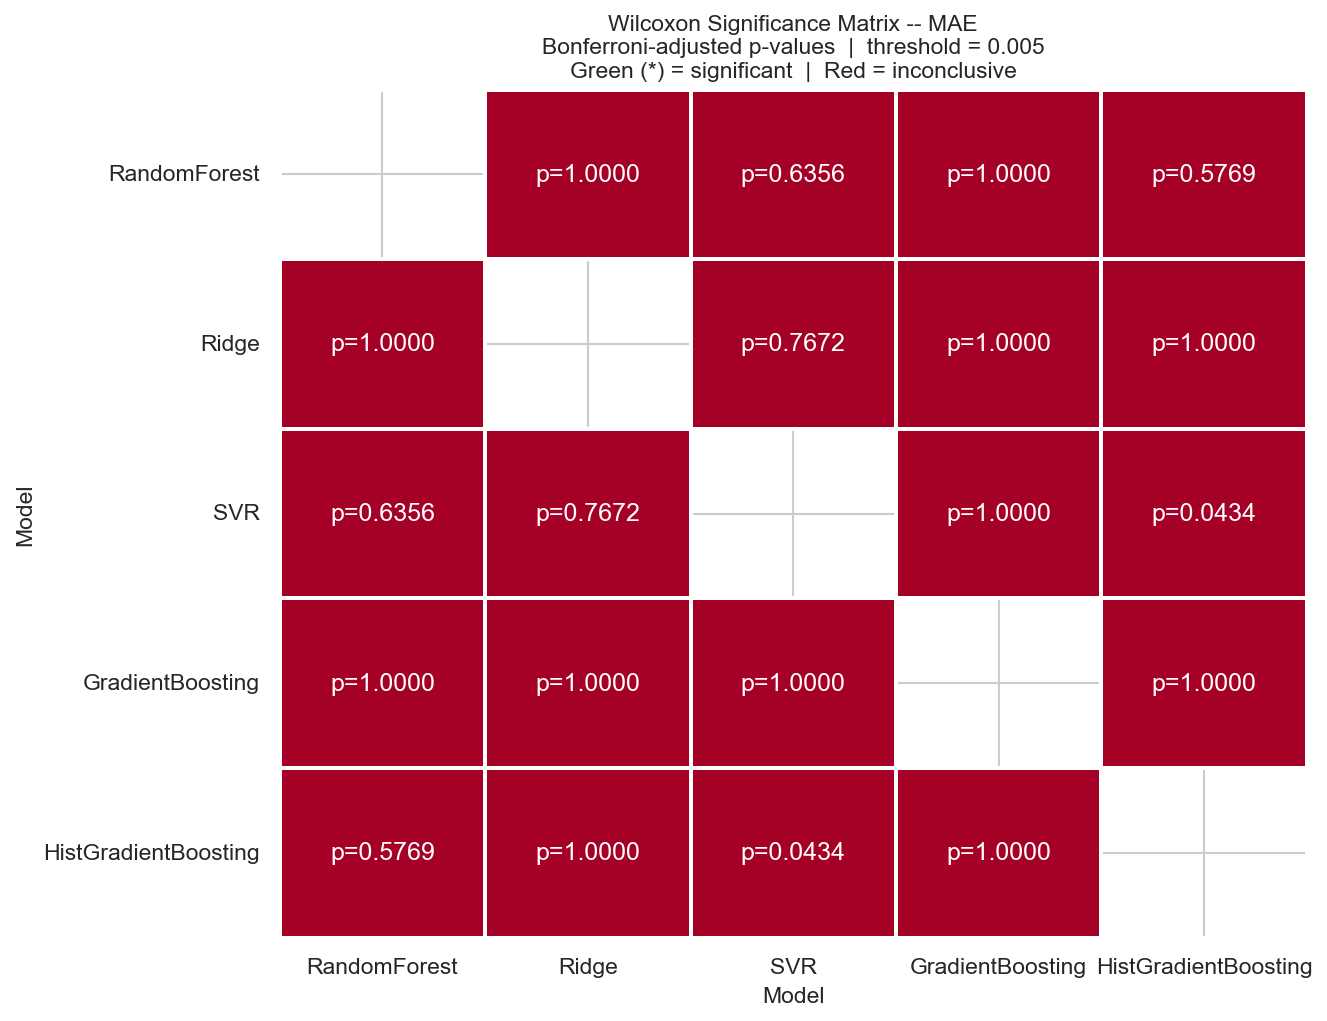
\includegraphics[width=0.7\textwidth]{../results/experiment_1_sig_matrix.png}
  \caption{Pairwise significance matrix for Experiment~1 model comparisons. All ten comparisons
  are inconclusive at the Bonferroni-corrected threshold of $\alpha = 0.005$.}
  \label{fig:exp1_sigmatrix}
\end{figure}

None of the ten pairwise comparisons reaches the Bonferroni-corrected threshold of 0.005. All ten
results must be characterised as inconclusive: the available data cannot establish whether any two
models differ in their ability to approximate the Anovator bodyAge score at the required level of
statistical confidence.

\subsection{Per-Prediction Error Distribution and Clinical Reliability}

Table~\ref{tab:exp1_reliability} presents the per-prediction absolute error distribution for
HistGradientBoosting across all 655 test predictions in the 30 folds.

\begin{table}[h]
  \centering
  \caption{Per-prediction absolute error distribution (HistGradientBoosting, 655 test predictions
  across 30 folds).}
  \label{tab:exp1_reliability}
  \begin{tabular}{lrr}
    \toprule
    \textbf{Tolerance} & \textbf{Predictions within tolerance} & \textbf{Percentage} \\
    \midrule
    $\leq 0.5$ years & 77 / 655  & 11.8\% \\
    $\leq 1.0$ years & 144 / 655 & 22.0\% \\
    $\leq 2.0$ years & 247 / 655 & 37.7\% \\
    $\leq 3.0$ years & 326 / 655 & 49.8\% \\
    \bottomrule
  \end{tabular}
\end{table}

The median absolute error across 655 individual predictions is 3.00 years; the 90th percentile is
6.84 years. These figures are substantially higher than the 2.43-year mean fold-level MAE reported
in Table~\ref{tab:exp1_results}. The discrepancy arises from the GroupShuffleSplit structure
interacting with the 103 records labelled ``Unknown'' in the name field. When the Unknown group
falls into a test fold, all 103 of its records are evaluated by a model trained exclusively on named
individuals, producing a sharp distribution shift that drives high errors in those folds.

\section{Experiment 2: Synthetic Data Ablation}

\subsection{Synthetic Data Fidelity}

The quality of the GMM-generated synthetic population was assessed by comparing its pairwise
correlation structure to that of the 158 real training records. The correlation matrix was computed
over all 79 shared numeric features. The mean absolute pairwise correlation difference between the
real and synthetic matrices is 0.0244, and the Frobenius norm of the difference matrix is 2.46 over
a $79 \times 79$ matrix (equivalent to a normalised value of 0.031 per feature). These figures
indicate that the GMM synthesis preserves inter-feature relationships closely.

\subsection{Performance by Regime and Model}

Table~\ref{tab:exp2_results} presents mean MAE with 95\% confidence intervals for all five models
under each of the three training regimes.

\begin{table}[h]
  \centering
  \caption{Experiment 2: Mean MAE (95\% CI) by model and training regime. All test evaluations
  use the same real held-out folds with true age\_gap labels.}
  \label{tab:exp2_results}
  \begin{tabular}{lrrr}
    \toprule
    \textbf{Model} & \textbf{RealOnly} & \textbf{RealPlusSynth} & \textbf{SynthOnly} \\
    \midrule
    HistGradientBoosting & 2.43 [2.09, 2.76] & 2.09 [1.85, 2.32] & 2.07 [1.84, 2.30] \\
    GradientBoosting     & 2.51 [2.19, 2.84] & 2.15 [1.93, 2.37] & 2.07 [1.85, 2.30] \\
    RandomForest         & 2.51 [2.18, 2.84] & 2.26 [2.05, 2.47] & 2.17 [1.93, 2.40] \\
    Ridge                & 2.48 [2.09, 2.87] & 2.39 [2.15, 2.63] & 3.23 [2.14, 4.31] \\
    SVR                  & 2.62 [2.30, 2.94] & 2.28 [2.06, 2.49] & 2.24 [2.02, 2.45] \\
    \bottomrule
  \end{tabular}
\end{table}

\begin{figure}[h]
  \centering
  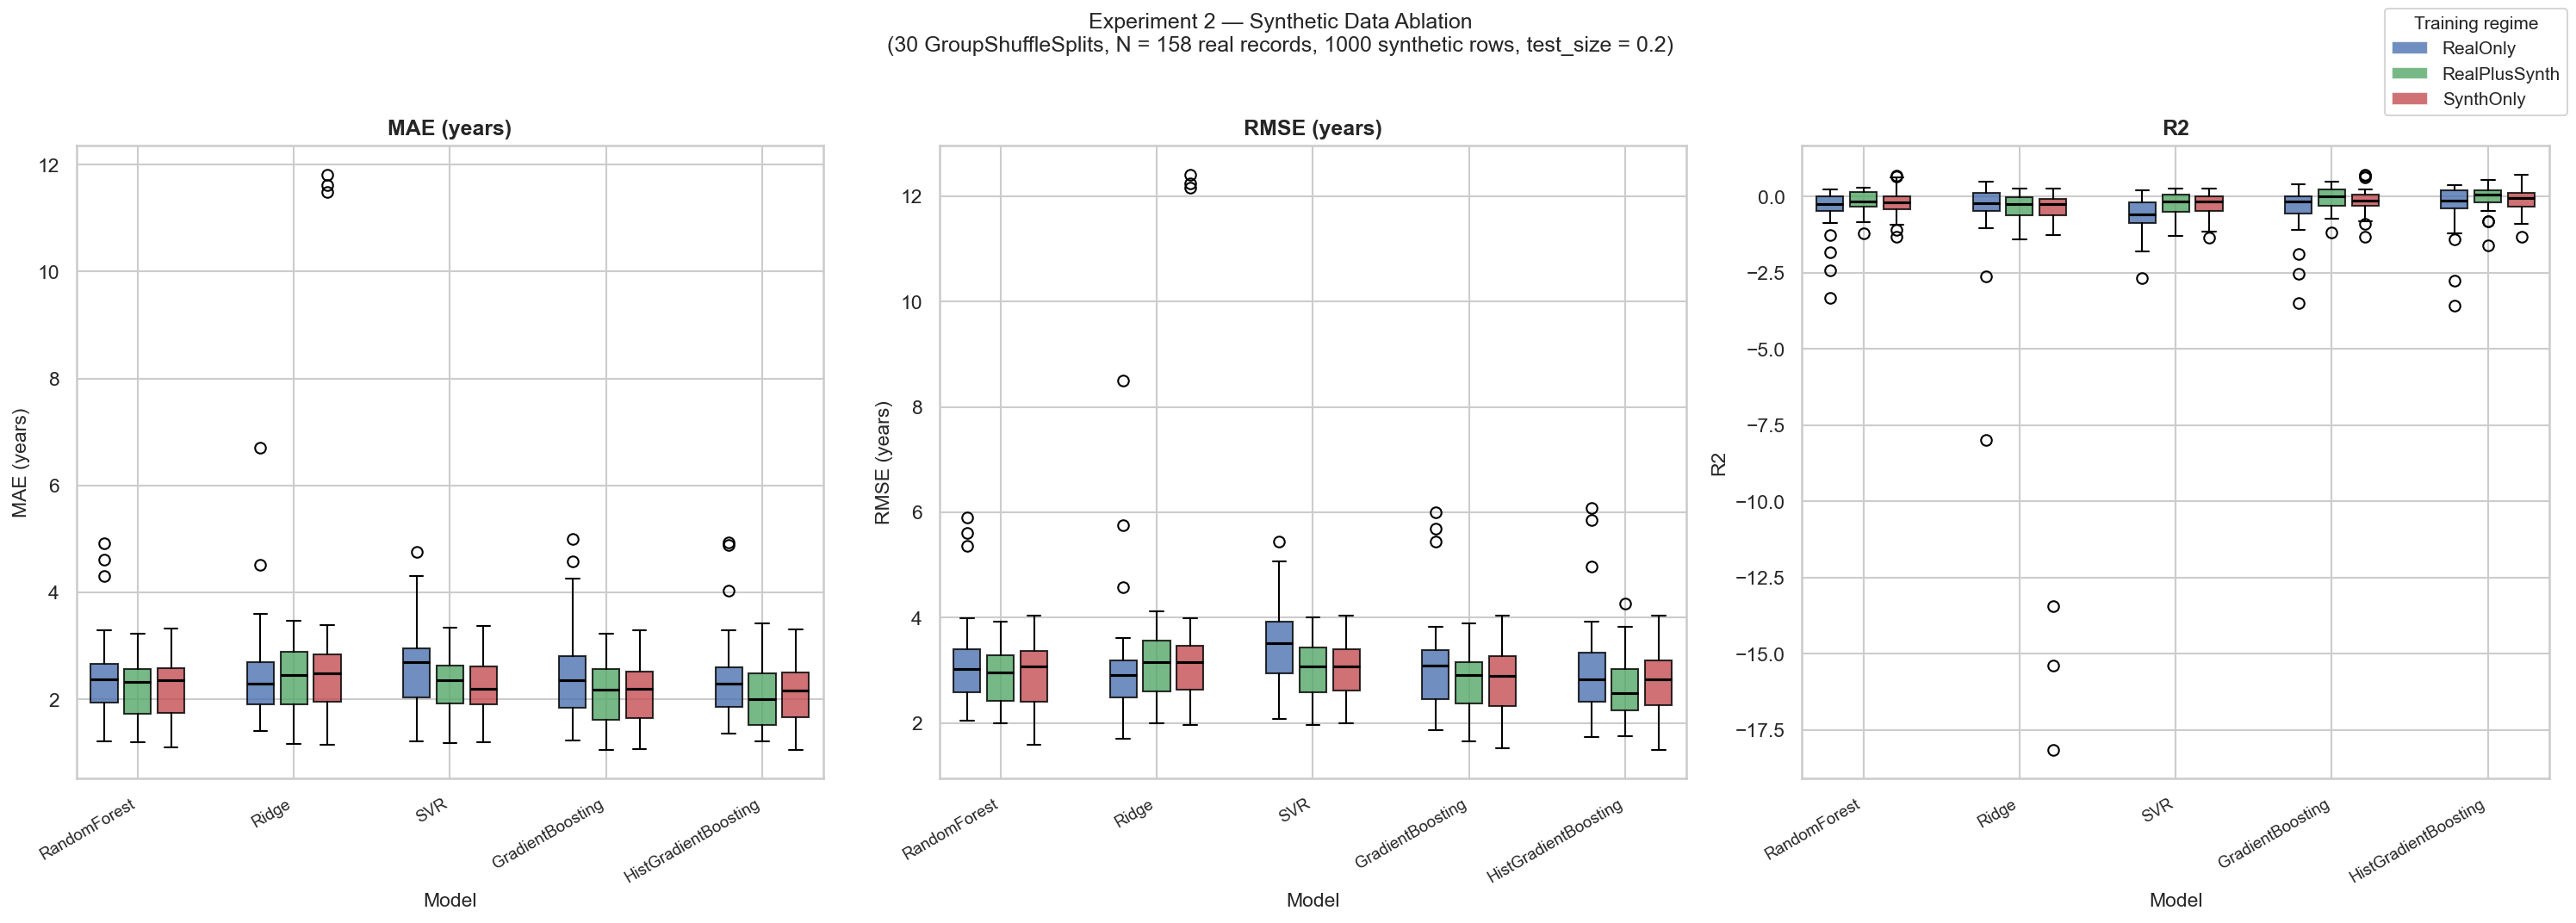
\includegraphics[width=0.85\textwidth]{../results/experiment_2_boxplot.png}
  \caption{Box plot of MAE distributions by training regime and model (Experiment~2). The Ridge
  SynthOnly distribution has a substantially wider spread and higher median than all other
  conditions.}
  \label{fig:exp2_boxplot}
\end{figure}

\begin{figure}[h]
  \centering
  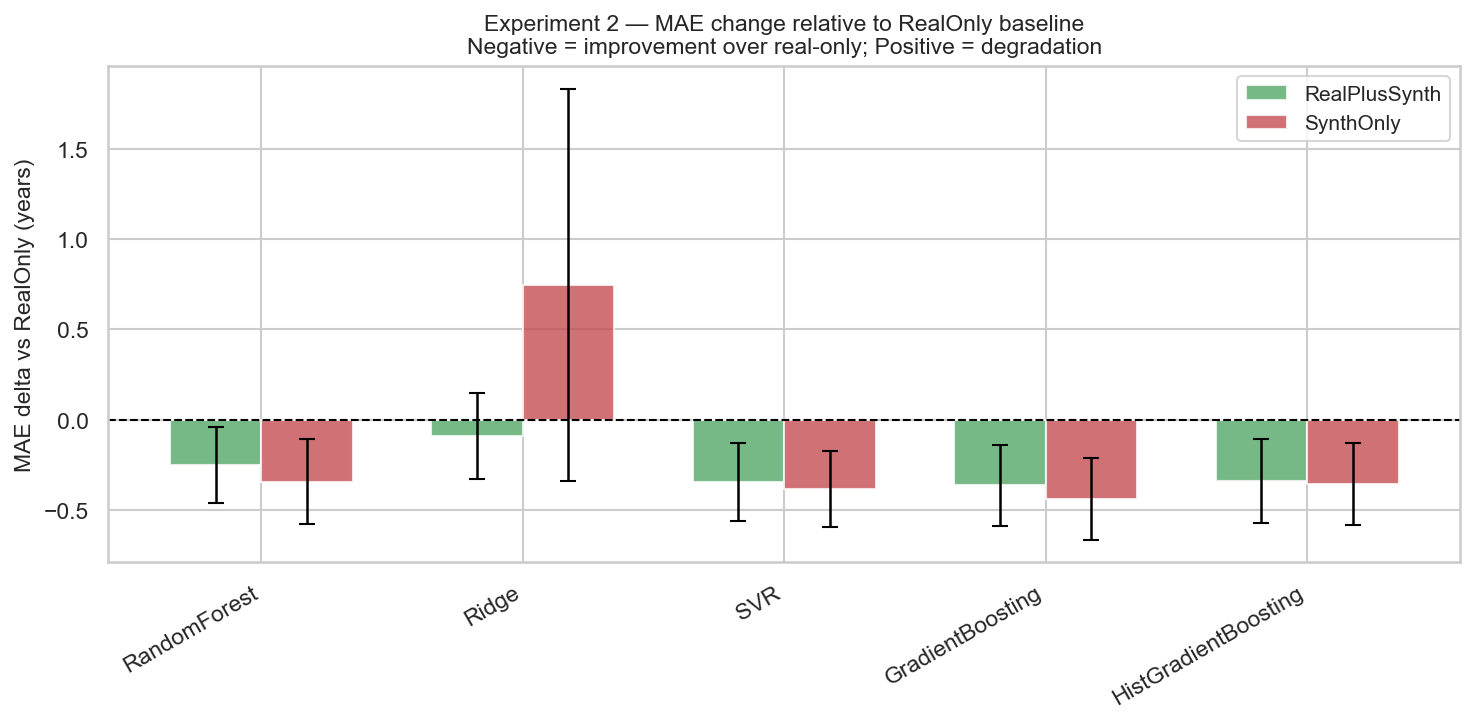
\includegraphics[width=0.75\textwidth]{../results/experiment_2_delta_plot.png}
  \caption{Mean MAE delta relative to the RealOnly baseline for each model under RealPlusSynth
  and SynthOnly training regimes (Experiment~2). Negative values indicate improvement over
  the RealOnly baseline.}
  \label{fig:exp2_delta}
\end{figure}

Under the RealPlusSynth regime, four of the five models show a reduction in mean MAE relative to
RealOnly, with improvements ranging from 0.09 years for Ridge to 0.36 years for
HistGradientBoosting. Ridge degrades substantially under the SynthOnly regime to a mean MAE of
3.23 years, the single largest deterioration observed across the entire experiment.

\subsection{Statistical Significance}

Table~\ref{tab:exp2_sig} presents the statistically significant pairwise comparisons from
Experiment~2 on MAE. Bonferroni correction is applied over three regime pairs per model, yielding
a corrected threshold of 0.0167.

\begin{table}[h]
  \centering
  \caption{Experiment 2: Significant Wilcoxon results for MAE (Bonferroni $\alpha = 0.0167$). Only
  comparisons reaching significance are shown; all remaining pairs are inconclusive.}
  \label{tab:exp2_sig}
  \begin{tabular}{llrrr}
    \toprule
    \textbf{Model} & \textbf{Regime A} & \textbf{Regime B} & \textbf{$p$ (raw)} & \textbf{$p$ (adjusted)} \\
    \midrule
    HistGradientBoosting & RealOnly & RealPlusSynth & $<0.000001$ & 0.000004 \\
    SVR                  & RealOnly & RealPlusSynth & 0.000003    & 0.000010 \\
    SVR                  & RealOnly & SynthOnly     & 0.000027    & 0.000081 \\
    RandomForest         & RealOnly & RealPlusSynth & 0.000111    & 0.000332 \\
    GradientBoosting     & RealOnly & RealPlusSynth & 0.000952    & 0.002855 \\
    \bottomrule
  \end{tabular}
\end{table}

Five comparisons reach significance. For HistGradientBoosting, RandomForest, GradientBoosting, and
SVR, the RealOnly versus RealPlusSynth comparison is statistically significant, with adjusted
$p$-values ranging from 0.000004 to 0.002855. No regime pair comparison reaches significance for
Ridge. The RealPlusSynth versus SynthOnly comparison is not significant for any model.

\section{Experiment 3: Feature Group Ablation}

\subsection{Performance by Feature Group}

Table~\ref{tab:exp3_results} presents mean MAE, RMSE, and $R^2$ with 95\% confidence intervals for
HistGradientBoosting under each of the four cumulative feature group conditions.

\begin{table}[h]
  \centering
  \caption{Experiment 3: Mean performance metrics (95\% CI) by feature group
  (HistGradientBoosting).}
  \label{tab:exp3_results}
  \small
  \resizebox{\textwidth}{!}{%
  \begin{tabular}{lrrrrrrrr}
    \toprule
    \textbf{Group} & \textbf{Feat.} & \textbf{MAE} & \textbf{MAE CI}
                   & \textbf{RMSE} & \textbf{RMSE CI}
                   & \textbf{$R^2$} & \textbf{$R^2$ CI} \\
    \midrule
    G1: Anthropometric + Metabolic & 63 & 2.39 & [2.05,\ 2.72] & 3.01 & [2.62,\ 3.40] & $-0.33$ & [$-0.66$,\ $-0.01$] \\
    G2: + Bioimpedance             & 73 & 2.42 & [2.07,\ 2.76] & 3.05 & [2.65,\ 3.46] & $-0.37$ & [$-0.72$,\ $-0.03$] \\
    G3: + Postural Risk            & 83 & 2.42 & [2.08,\ 2.76] & 3.06 & [2.67,\ 3.46] & $-0.37$ & [$-0.71$,\ $-0.04$] \\
    G4: + Joint Angles (full)      & 88 & 2.43 & [2.09,\ 2.76] & 3.05 & [2.66,\ 3.44] & $-0.36$ & [$-0.70$,\ $-0.03$] \\
    \bottomrule
  \end{tabular}}
\end{table}

\begin{figure}[h]
  \centering
  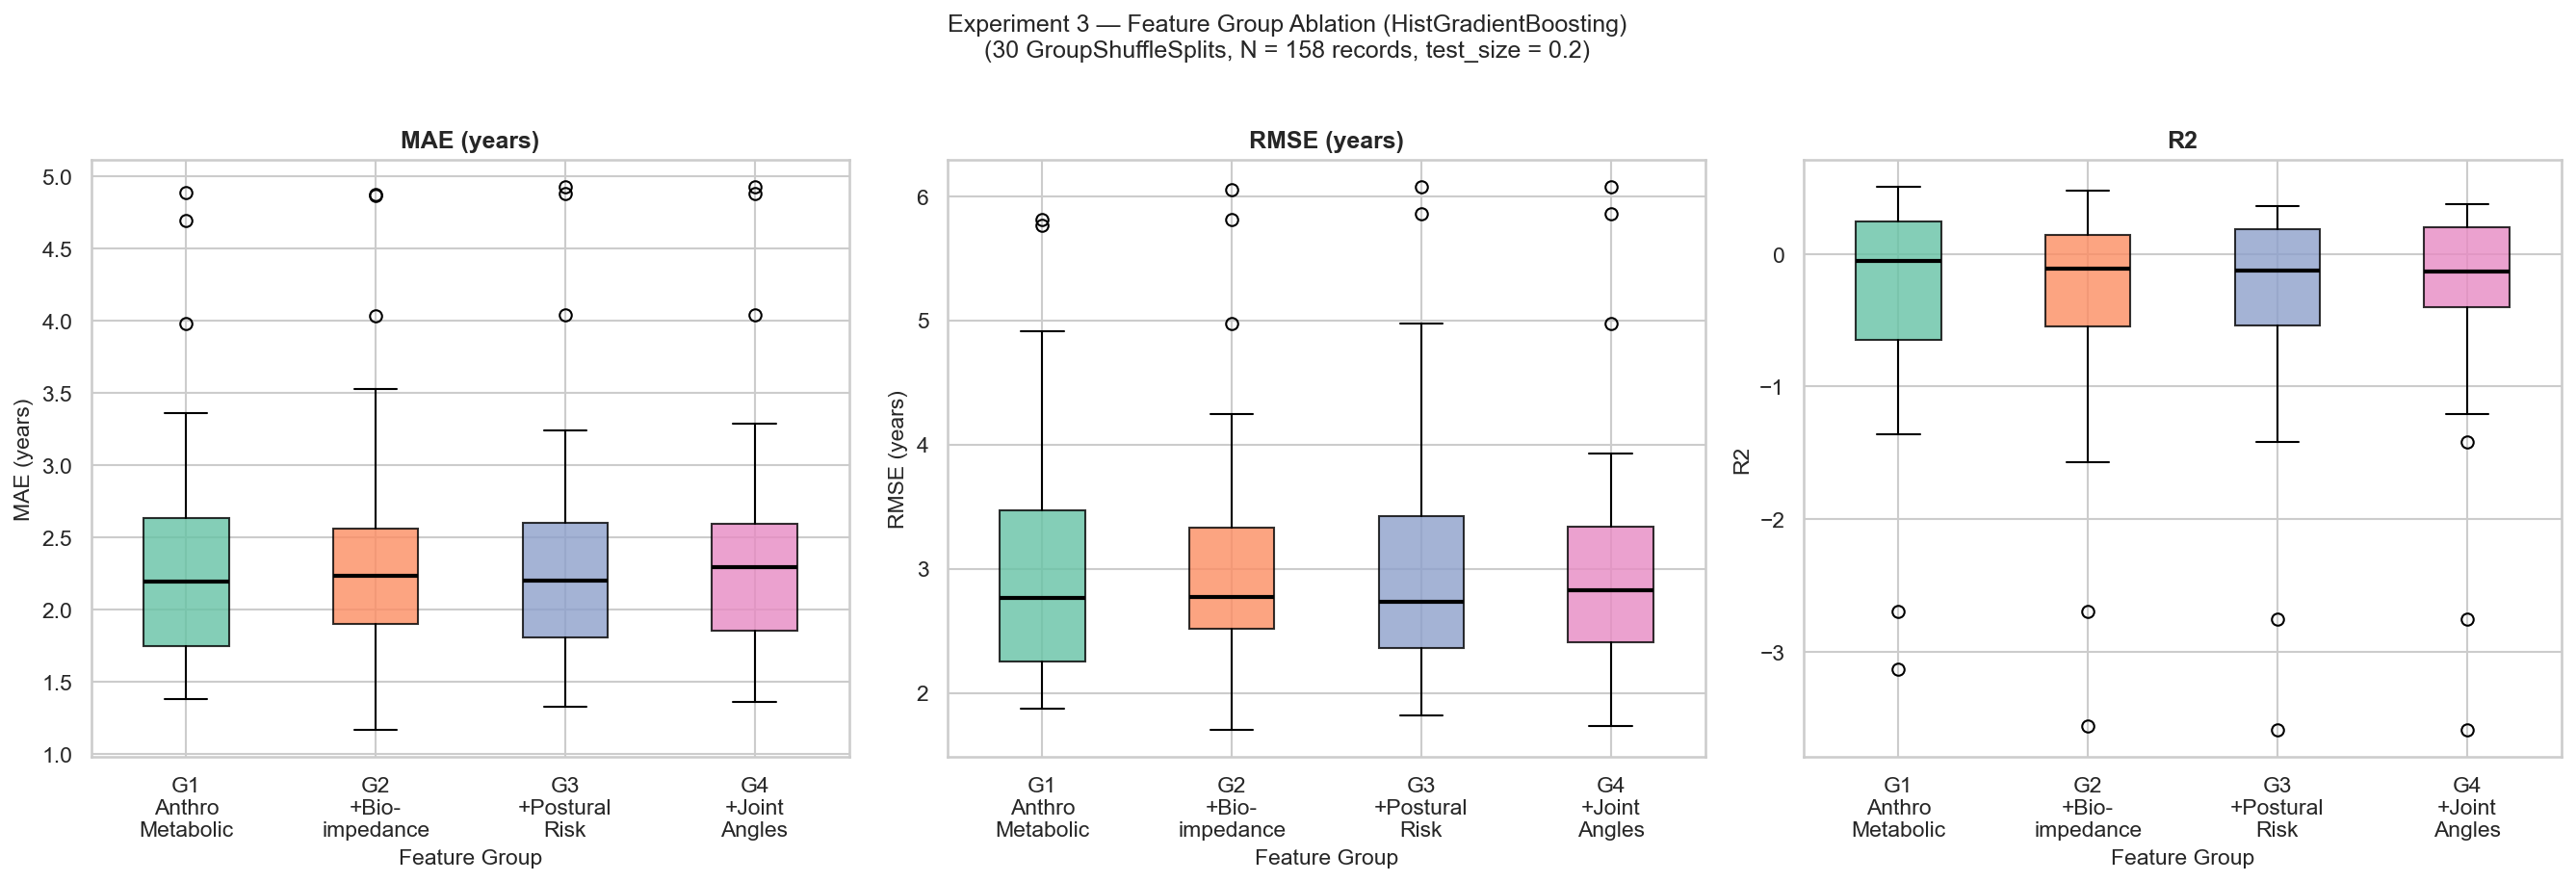
\includegraphics[width=0.75\textwidth]{../results/experiment_3_boxplot.png}
  \caption{Box plot of MAE distributions by cumulative feature group (Experiment~3,
  HistGradientBoosting).}
  \label{fig:exp3_boxplot}
\end{figure}

\begin{figure}[h]
  \centering
  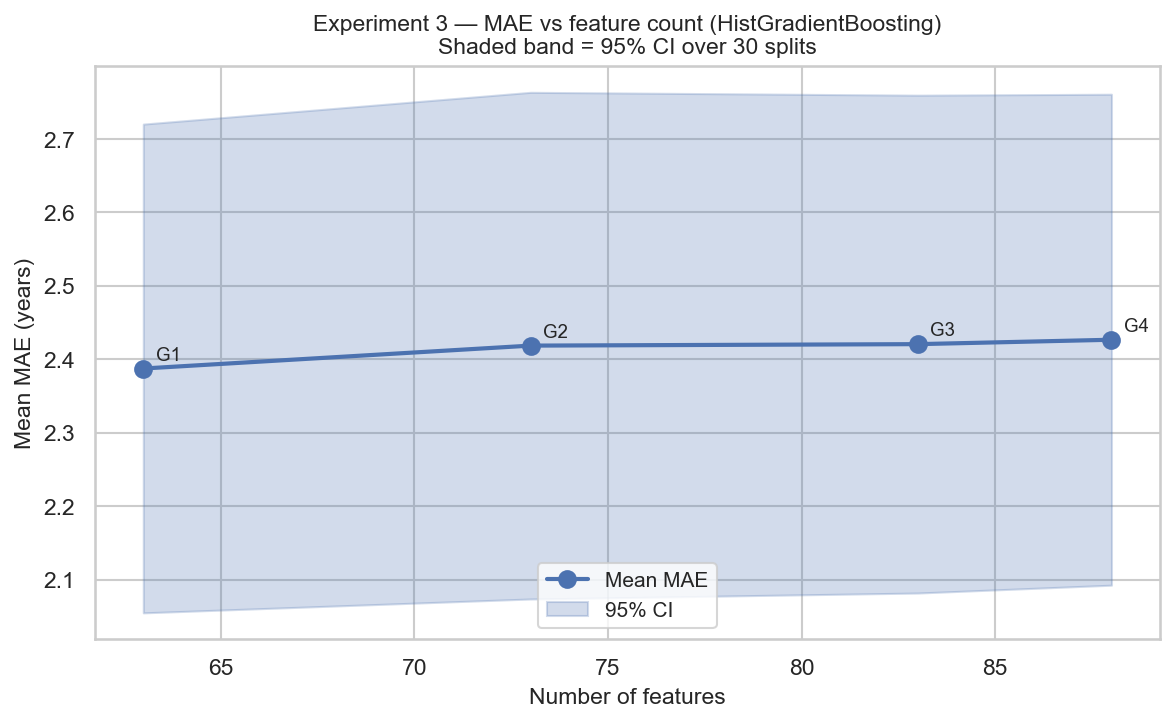
\includegraphics[width=0.7\textwidth]{../results/experiment_3_learning_curve.png}
  \caption{Mean MAE by cumulative feature group (Experiment~3). Error bars represent 95\%
  confidence intervals across 30 cross-validation folds. The monotonic increase from G1 to G4 is
  not statistically significant.}
  \label{fig:exp3_mae}
\end{figure}

The anthropometric and metabolic group (G1) achieves the lowest mean MAE at 2.39 years. Each
successive addition of a feature group is associated with a marginal increase in mean MAE. The
total difference between the 63-feature group and the full 88-feature set is 0.04 years.

\subsection{Statistical Significance}

Table~\ref{tab:exp3_sig} presents the Wilcoxon signed-rank test results for all six group pairs
on MAE, with Bonferroni-corrected $p$-values and the corrected significance threshold of 0.0083.

\begin{table}[h]
  \centering
  \caption{Experiment 3: Wilcoxon signed-rank test results for MAE (Bonferroni $\alpha = 0.0083$).}
  \label{tab:exp3_sig}
  \begin{tabular}{llrrr}
    \toprule
    \textbf{Group A} & \textbf{Group B} & \textbf{$p$ (raw)} & \textbf{$p$ (adjusted)} & \textbf{Sig.} \\
    \midrule
    G1: Anthropometric + Metabolic & G3: + Postural Risk   & 0.2207 & 1.0000 & No \\
    G1: Anthropometric + Metabolic & G4: + Joint Angles    & 0.2129 & 1.0000 & No \\
    G1: Anthropometric + Metabolic & G2: + Bioimpedance    & 0.2710 & 1.0000 & No \\
    G2: + Bioimpedance             & G4: + Joint Angles    & 0.4280 & 1.0000 & No \\
    G3: + Postural Risk            & G4: + Joint Angles    & 0.5481 & 1.0000 & No \\
    G2: + Bioimpedance             & G3: + Postural Risk   & 0.5699 & 1.0000 & No \\
    \bottomrule
  \end{tabular}
\end{table}

None of the six pairwise comparisons reaches the Bonferroni-corrected threshold of 0.0083. All six
comparisons are therefore inconclusive.


% =============================================================================
\chapter{Discussion}
% =============================================================================

\section{The Null Result in Experiment 1 Is a Finding, Not a Failure}

The absence of statistical significance across all ten pairwise model comparisons in Experiment~1
is the most important single result in this thesis and must be stated precisely. The Wilcoxon
signed-rank test on 30 paired fold observations, corrected for ten simultaneous comparisons at
$\alpha = 0.005$, found no evidence that any two of the five models differ in their ability to
approximate the Anovator bodyAge score. The adjusted $p$-value for the closest comparison ---
SVR versus HistGradientBoosting --- was 0.043, an order of magnitude above the corrected threshold.

This result does not mean the models are equivalent. Claiming equivalence from a non-significant
Wilcoxon test would commit the fundamental error of accepting the null hypothesis. What the result
means is that the study, as constituted, cannot resolve the performance difference between these
models with the required statistical confidence. The confidence intervals reported in
Table~\ref{tab:exp1_results} span approximately 0.65 to 0.78 years --- a range that is large
relative to the mean differences between models, which are all below 0.20 years.

The finding has scientific content precisely because it is unexpected. The fact that Ridge
regression achieves mean MAE within 0.05 years of HistGradientBoosting suggests either that the
predictive information in these 88 features is largely captured by linear combinations of those
features, implying that Anovator's proprietary formula may itself be approximately linear in the
inputs; or that the test folds are too small to discriminate non-linear signal from noise at this
dataset scale.

\section{Synthetic Augmentation Helps Ensemble Methods and Damages Ridge}

Experiment~2 produces the strongest statistical results in the study. The mechanism is interpretable
within the teacher-student framework. Tree-based ensemble methods and kernel SVMs benefit from
larger training sets because they rely on local density estimation or partitioning that becomes more
reliable as the coverage of the input space increases. The 1000 synthetic records fill gaps in the
biometric input space that the 53 individuals in the real dataset leave sparsely covered.

Ridge regression is the exception. Under the SynthOnly regime, Ridge's mean MAE rises to 3.23 years
from a RealOnly baseline of 2.48 years --- a 30\% degradation. This behaviour is a direct consequence
of the pseudo-label distribution: the production model's predictions on the synthetic records have a
standard deviation of 1.91 years compared to 3.30 years in the real label distribution. Linear
models fit their coefficients to minimise squared error across the training distribution; when the
training distribution artificially compresses the label variance, the fitted linear model learns a
relationship calibrated to a narrower output range than the true target.

The RealPlusSynth versus SynthOnly comparison is not significant for any model, meaning that the
real training records cannot be shown to add distinguishable value over the synthetic corpus alone
under the available statistical power.

\section{Feature Group Saturation and What It Implies About Anovator's Formula}

The most counterintuitive finding in the study is that the 63-feature anthropometric and metabolic
group alone achieves lower mean MAE (2.39 years) than any larger feature set, including the full
88-feature model (2.43 years). The most important interpretation concerns the structure of the
Anovator formula itself. If the formula places low or negligible weight on bioimpedance raw values,
postural camera risk scores, and joint angles in favour of anthropometric and metabolic measurements,
then a model attempting to reverse-engineer the formula would find no additional predictive
information in those feature groups beyond what the base group already captures.

The operational implication is consistent: at this data scale, there is no statistical justification
for preferring the full 88-feature model over the 63-feature anthropometric and metabolic subset.

\section{SHAP Feature Importance: Physiological Interpretation}

Global SHAP values reveal a pronounced concentration of predictive weight in anthropometric and
metabolic features. Waist circumference (\texttt{wc}) is the single dominant predictor with a mean
absolute SHAP value of 0.69 years, more than twice that of any other feature. Its dominance is
consistent with its likely role as a primary input to the Anovator bodyAge formula: central obesity
is the biometric signal most directly linked to the cardiometabolic outcomes that commercial
biological age scores typically aim to capture.

The second and third most influential features --- \texttt{aerobicGoal} and \texttt{agility} ---
warrant a caveat. \texttt{AerobicGoal} is an Anovator-computed training recommendation, not a raw
biometric measurement, meaning the surrogate model has partially learned to use Anovator's own
intermediate outputs as predictors of the final score, which is expected in a reverse-engineering
setting but limits physiological interpretability. Intra-abdominal fat (\texttt{inFat}) and BMI
follow as the fourth and sixth most important features respectively. The first bioimpedance feature
(\texttt{r20LeftLeg}) appears at rank five, and the first joint angle feature appears at rank
eleven --- well below the anthropometric and metabolic cluster. This gradient directly supports the
interpretation that Anovator's formula draws its predictive structure primarily from body
composition, fitness, and metabolic measurements.

\section{The Underpowered Wilcoxon Caveat and Its Scope}

The statistical power limitation described in Section~\ref{sec:power} applies differently across
the three experiments. In Experiment~1, it is binding: all ten adjusted $p$-values are well above
the corrected threshold. In Experiment~2, it is not binding for the five significant comparisons,
which reach adjusted $p$-values as low as 0.000004; the limitation is relevant only for the
non-significant regime comparisons. In Experiment~3, it is clearly binding: the lowest raw
$p$-value observed is 0.21, a value that would not reach even the uncorrected 0.05 threshold.

None of these observations are apologetic qualifications of a study that failed to find what it was
looking for. Underpowered tests that return non-significant results are honest results.

\section{Known Limitations and Their Bearing on Interpretation}

The four limitations documented in Section~\ref{sec:limitations} bear on the interpretation of results as follows.
The sentinel encoding of \texttt{sportSafeRisk} and \texttt{sportLevel} may introduce systematic
artefacts into the learned feature space but does not affect the comparability of results across
experiments, since all conditions share the same encoding. The near-constant imputed features
inflate the nominal dimensionality without proportional contribution to predictive performance. The
redundant \texttt{aggregated\_postural\_index} has negligible practical effect on tree-based models
due to their tolerance for collinear features. Finally, the single-centre, 53-individual dataset
means that all findings must be characterised as an analysis of the reverse-engineering problem
within this specific dataset rather than a generalisation claim at population scale.

\section{Synthesis}

Taken together, the three experiments produce a coherent picture. The five models are statistically
indistinguishable on the real-data-only approximation task, suggesting that the predictive
information available in the 88 features is largely captured by their linear structure and by the
anthropometric and metabolic subset in particular. Synthetic augmentation through teacher-student
pseudo-labelling produces statistically significant improvements for ensemble methods and SVR,
indicating that the 53-individual training corpus is the primary constraint on approximation
quality. Ridge's failure under the SynthOnly regime provides a clear case study in the conditions
under which synthetic augmentation is contraindicated.


% =============================================================================
\chapter{Conclusion}
% =============================================================================

\section{Summary of Findings}

Experiment~1 evaluated five regression algorithms on their ability to predict the Anovator age gap
from the full 88-feature biometric set. HistGradientBoosting achieved the lowest mean MAE at
2.43 years (95\% CI [2.09, 2.76]), with SVR the weakest at 2.62 years. The remaining three models
clustered within 0.04 years of each other. None of the ten pairwise Wilcoxon signed-rank tests
reached the Bonferroni-corrected significance threshold of 0.005; all ten comparisons must be
reported as inconclusive.

Experiment~2 tested three training regimes. Under the RealPlusSynth regime, four of the five
models showed statistically significant improvement over RealOnly training, with adjusted $p$-values
ranging from 0.000004 to 0.002855 and mean MAE reductions of 0.09 to 0.36 years. Ridge was the
exception: its mean MAE under the SynthOnly regime rose to 3.23 years from a baseline of 2.48
years, a 30\% degradation explained by the mismatch between compressed pseudo-label variance
(standard deviation 1.91 years) and the true label variance (standard deviation 3.30 years).

Experiment~3 applied a cumulative feature group ablation to HistGradientBoosting. Counterintuitively,
the 63-feature anthropometric and metabolic base group alone achieved the lowest mean MAE at
2.39 years, with each successive addition of features associated with a marginal increase in error.
None of the six pairwise comparisons reached the Bonferroni-corrected threshold of 0.0083.

\section{Answers to the Research Sub-Questions}

The first sub-question asked which regression algorithm best approximates the Anovator age gap and
whether any performance difference is statistically certifiable. The answer is two-part:
HistGradientBoosting is the numerically preferred model by heuristic ranking, and no algorithm can
be certified as statistically superior to the others at the available sample size.

The second sub-question asked whether GMM synthetic augmentation improves approximation quality and
for which model classes. For ensemble methods and SVR the answer is yes, with statistically
significant improvements under the RealPlusSynth regime. For Ridge the answer is no: synthetic
augmentation through teacher-student pseudo-labelling is contraindicated when pseudo-label variance
is substantially compressed relative to the real target distribution.

The third sub-question asked which biometric feature groups carry independent predictive information.
No statistical evidence exists for independent predictive contribution from bioimpedance, postural
risk, or joint angle features beyond the anthropometric and metabolic base, but equivalence cannot
be asserted either --- all comparisons are inconclusive at the available sample size.

\section{Limitations}

Four dataset and methodological limitations are documented in full in Section~\ref{sec:limitations}. In brief: two
features use the integer $-1$ as a sentinel for missing data and are treated as continuous numeric
inputs; five features with missingness above 88\% become near-constants after imputation; the
derived feature \texttt{aggregated\_postural\_index} is arithmetically redundant within the postural
risk group; and the Wilcoxon signed-rank test at Bonferroni-corrected thresholds has limited power
with 30 paired observations. The 53-individual, single-centre dataset is the binding constraint
throughout.

\section{Future Work}

Dataset expansion is the highest-priority item. Collecting Anovator scan records from additional
health centres would reduce single-gym bias, increase statistical power in all three experiment
types, and enable time-based evaluation splits that the current corpus cannot support. Sentinel value
re-encoding for \texttt{sportSafeRisk} and \texttt{sportLevel} is the most contained and
highest-impact preprocessing fix available. Alternative synthetic generation methods including CTGAN,
TVAE, and Gaussian copula approaches should be evaluated once the real dataset exceeds approximately
500 records. Imputation strategy sensitivity analysis using KNN or MICE imputation would test
whether results are robust to the modelling choice applied to features with high missingness rates.
Longitudinal evaluation using time-based splits would test whether the models generalise across time
as well as across individuals. Formal power analysis prior to any dataset expansion effort would
quantify the sample size required to detect effect sizes of practical relevance at the
Bonferroni-corrected thresholds used here.


% =============================================================================
% Appendices
% =============================================================================
\begin{appendices}

\chapter{Ethical Considerations}

\section{Data Classification Under GDPR}

The dataset used in this study consists of Anovator body scan records collected from clients of
Zdravoletie. Under the General Data Protection Regulation (EU) 2016/679, this data falls into two
protected categories. First, the name field constitutes personal data under Article 4(1), as it
directly identifies natural persons. Second, the biometric and health measurement fields ---
including body composition percentages, impedance values, postural risk scores, blood pressure,
heart rate, vision acuity, and the derived bodyAge score --- constitute special category data under
Article 9(1), specifically data concerning health.

Of the 158 records in the dataset, 103 carry the name value ``Unknown''. The remaining 50 records
carry values that appear to be dates of birth encoded as six-digit strings, which are pseudonyms
rather than true names but remain linkable to individuals within the clinic's operational records.
The \texttt{original\_url} and \texttt{id} fields contain Anovator platform identifiers that could
be used to retrieve additional personal data; these fields were not used in any modelling or
analysis and are excluded from the model feature set.

\section{Consent Assumptions}

The data were collected in the course of normal clinical operations at Zdravoletie. It is assumed
that Zdravoletie's standard client intake process includes consent to collection and processing of
biometric data for health assessment purposes. However, this study did not verify whether clients
were specifically informed that their scan data would be used for machine learning research or
shared with a student researcher. This represents a gap relative to the Article 9(2)(a) explicit
consent standard for research use of special category data.

\section{Data Handling in This Study}

The dataset was transferred to the researcher's local development environment as a CSV export and
was not uploaded to any public repository, cloud storage service, or third-party platform during
analysis. All modelling, experiment scripts, and visualisations were executed locally. The Streamlit
dashboard does not transmit client data to external servers; all prediction and SHAP computation
runs client-side within the Streamlit session. Model artifact files (\texttt{.joblib}) stored in
the repository contain only fitted model parameters and no training records.

\section{Requirements for Production Deployment}

A production deployment of the Streamlit dashboard or any successor system would require the
following before going live: a Data Protection Impact Assessment (DPIA) under Article 35 GDPR;
explicit informed consent forms covering research and analytical use of scan data; a Data Processing
Agreement under Article 28 GDPR with any cloud hosting provider; authentication restricting access
to authorised clinic staff; audit logging of record access; and a documented data retention policy
for compliance with Article 17 erasure requests.

\end{appendices}

% =============================================================================
% Bibliography
% =============================================================================
\bibliography{references}

\end{document}
